\documentclass[11pt,a4paper]{article}
\usepackage[utf8]{inputenc}
\usepackage[french,francais]{babel}
\usepackage{fontenc}
\usepackage{amsmath}
\usepackage{amsfonts}
\usepackage{amssymb}
\usepackage{graphicx}
\usepackage{geometry}
\usepackage{caption}
\usepackage{subcaption}
\usepackage{numprint}
\usepackage[hyphens]{url}
\usepackage{listingsutf8}
\usepackage{mcode}
\usepackage{float}
\usepackage{color}
\usepackage{fancyhdr}
\usepackage{lastpage} % Required to determine the last page for the footer
\usepackage{extramarks} % Required for headers and footers

\geometry{
	body={160mm,250mm},
	left=25mm,top=25mm,
	headheight=7mm,
	headsep=4mm,
	marginparsep=4mm,
	marginparwidth=21mm}
\lstset{
		inputencoding=latin1,
		language=Matlab,
		%frame=single,
		basicstyle=\normalsize, % ou ça==> basicstyle=\scriptsize,
numbers=left,
aboveskip={1.5\baselineskip},
columns=fullflexible,
showstringspaces=false,
extendedchars=true,
breaklines=true,
showtabs=false,
showspaces=false,
showstringspaces=false,
		literate=
  {á}{{\'a}}1 {é}{{\'e}}1 {í}{{\'i}}1 {ó}{{\'o}}1 {ú}{{\'u}}1
  {Á}{{\'A}}1 {É}{{\'E}}1 {Í}{{\'I}}1 {Ó}{{\'O}}1 {Ú}{{\'U}}1
  {à}{{\`a}}1 {è}{{\`e}}1 {ì}{{\`i}}1 {ò}{{\`o}}1 {ù}{{\`u}}1
  {À}{{\`A}}1 {È}{{\'E}}1 {Ì}{{\`I}}1 {Ò}{{\`O}}1 {Ò}{{\`U}}1
  {ä}{{\"a}}1 {ë}{{\"e}}1 {ï}{{\"i}}1 {ö}{{\"o}}1 {ü}{{\"u}}1
  {Ä}{{\"A}}1 {Ë}{{\"E}}1 {Ï}{{\"I}}1 {Ö}{{\"O}}1 {Ü}{{\"U}}1
  {â}{{\^a}}1 {ê}{{\^e}}1 {î}{{\^i}}1 {ô}{{\^o}}1 {û}{{\^u}}1
  {Â}{{\^A}}1 {Ê}{{\^E}}1 {Î}{{\^I}}1 {Ô}{{\^O}}1 {Û}{{\^U}}1
  {œ}{{\oe}}1 {Œ}{{\OE}}1 {æ}{{\ae}}1 {Æ}{{\AE}}1 {ß}{{\ss}}1
  {ç}{{\c c}}1 {Ç}{{\c C}}1 {ø}{{\o}}1 {å}{{\r a}}1 {Å}{{\r A}}1}


\pagestyle{fancy}
\lhead{\AuthorName} % Top left header
\chead{\Course} % Top center header
\rhead{\Date} % Top right header
\lfoot{\lastxmark} % Bottom left footer
\cfoot{} % Bottom center footer
\rfoot{\ \thepage\ / 	\pageref{LastPage}} % Bottom right footer
\renewcommand\headrulewidth{0.4pt} % Size of the header rule
\renewcommand\footrulewidth{0.4pt} % Size of the footer rule

\newcommand{\Course}{} % Course/class
\newcommand{\AuthorName}{Herrier L., Juckler C., Musuvaho G., Nyssens S.} % Your name
\newcommand{\Date}{EPHEC - Décembre 2014}


\author{Herrier Lucie \and Juckler Christian \and Musuvaho Grace \and Nyssens Sylvain}
\date{\today}

\begin{document}
\title{
\parbox{15cm}
{
\includegraphics[width=4cm]{ephec.png} \\ 
  Louvain-la-neuve\\
  \vspace{3cm}
	\begin{center}\sf\bfseries\Huge
		\rule{15cm}{1pt}
		\medskip
		Traitement de signal\\
		\huge Projet - Accordeur\\
		\vspace{.5cm}
		\Large Rapport de projet
		\vspace{.5cm}
		\rule{15cm}{1pt}
		\large 3TL1
	\end{center}
	\vspace{3cm}
}} 
\maketitle
\thispagestyle{empty}
\newpage
\mbox{}
\thispagestyle{empty}
\newpage
\setcounter{page}{1}
\tableofcontents
\newpage
\mbox{}
\thispagestyle{empty}
\newpage
\section{Introduction}
Dans le cadre du cours de travaux pratiques de traitement de signal, nous avons dû réaliser un projet mettant en application nos acquis. Notre groupe a choisi de créer un accordeur de guitare. Celui-ci a été codé à l'aide de Matlab, l'outil utilisé lors des exercices à réaliser durant le cours. Ce rapport présente tout d'abord en quelques lignes en quoi consistait le projet. Nous expliquons par la suite la méthodologie que nous avons utilisée, et nous apportons des idées d'améliorations possibles pour notre accordeur. Enfin, chaque membre du groupe apporte sa conclusion personnelles concernant ce projet.
\section{Présentation du projet}
Le projet que nous avons réalisé est un accordeur de guitare. Celui-ci a été codé à l'aide du logiciel utilisé lors des TPs, Matlab. Nous avons choisi d'implémenter une interface graphique, plus intuitive à utiliser. Celle-ci propose d'accorder sa guitare selon plusieurs accords fréquemment utilisés. La figure~\ref{interface} montre l'interface utilisateur de l'accordeur.

\begin{figure}[H]
\centering
\begin{subfigure}[b]{7cm}
	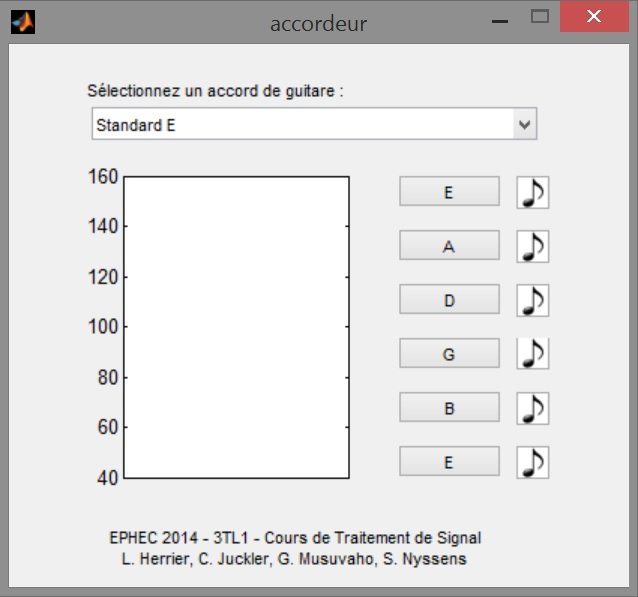
\includegraphics[width=6cm]{accordeur.jpg}
	\caption{Accordeur au démarrage}
\end{subfigure}
\begin{subfigure}[b]{7cm}
	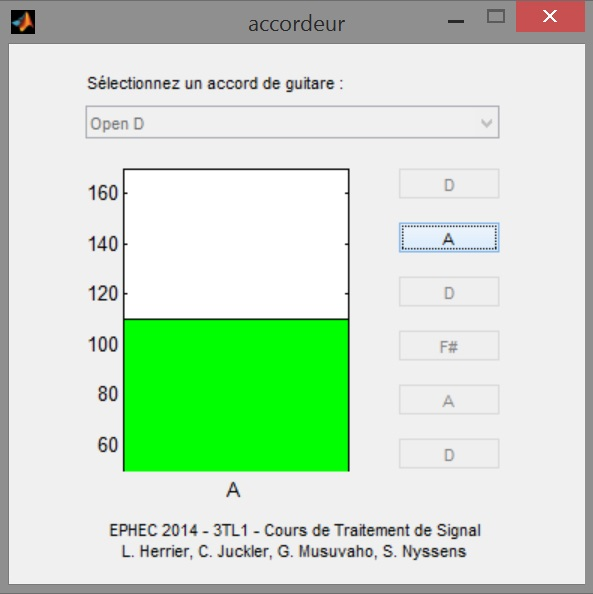
\includegraphics[width=6cm]{accordeurOn.jpg}
	\caption{Accordeur en train d'accorder}
\end{subfigure}
\caption{Interface utilisateur}
\label{interface}
\end{figure}

On peut voir sur les images ci-dessus la manière dont nous avons composé notre accordeur. Dans le haut de la fenêtre se trouve le menu de sélection des accords. Nous proposons divers accords fréquents pour la guitare : 
\begin{itemize}
\item L'accordage classique en\textit{ E}
\item Le \textit{Drop D}
\item L'\textit{Open D}
\item L'\textit{Open G}
\item L'accordage en \textit{quartes}
\end{itemize}
Les boutons de droite représentent les notes composant l'accord. Celui du dessus correspond à la corde du dessus lorsqu'on tient une guitare, autrement dit la note la plus grave. Enfin, le grand rectangle à gauche sert à visualiser si la corde de la guitare sélectionnée est bien accordée ou non. Le code couleur utilisé est classique : vert si la corde est correctement accordée, à 2Hz près, jaune-orange si la corde est trop haute ou trop basse à 15Hz près, et rouge si elle est hors des limites précédentes.\\

Lorsqu'une note est sélectionnée pour être accordée, un timer de 5 secondes s'enclenche. Il est possible pendant ce temps de jouer la corde pour l'accorder. De plus, les autres notes sont bloquées, ainsi que la sélection des accords, afin d'éviter les conflits.

\section{Méthodologie utilisée}
Lors de la réalisation de notre accordeur, nous sommes passés par plusieurs étapes avant d'arriver au produit actuel. Cette partie du rapport explique ces différentes phases de développement, ainsi que les difficultés rencontrées au cours de celles-ci.\\

En premier lieu, nous avons tout d'abord cherché à enregistrer un son dans Matlab. En effet, nous voulions pouvoir visualiser le spectre fréquentiel de l'enregistrement du son produit par une corde de guitare sur une durée déterminée.
Après plusieurs tentatives, nous y sommes arrivé.
Nous nous sommes vite rendu compte qu'il y avait un problème dans notre analyse.
Nous avons sous-estimé la puissance des harmoniques.
Lors de nos test, nous travaillions avec un logiciel capable de simuler un diapason et une guitare.
Avec le diapason, nous n'avions aucun doute sur notre approche.
Mais avec la guitare, nous avons remarqué que les harmoniques étaient plus puissante que la fréquence fondamentale.\\

Dans un deuxième temps, nous avons cherché à éliminer les harmoniques.
Pour ce faire, nous avons analysé les différents accords existants.
Il en a résulté que nous pouvions nous passer des fréquences au-delà de \numprint[Hz]{500}.
Ensuite, nous avons cherché à limiter la représentation graphique autour de la fréquence cherchée.
Chaque note possède sa propre fréquence, il n'est pas compliqué de borner les fréquences représentables sur le graphique.\\

Dans un troisième temps, nous avons réfléchi à une façon de stocker les différents accords existants en associant les notes avec leur fréquence respective.
Pour ce faire, nous sommes partis d'un La \numprint[Hz]{440} afin de générer la gamme de la 3ème octave. À partir de cette gamme, nous avons pu calculer les fréquences des notes pour les différents accords.

Parallèlement, nous avons commencé une interface graphique plus intuitive pour l'utilisateur.
Cette première interface affichait une zone d'accordage pour une fréquence fixée.
Avec cette interface, nous pouvions analyser une note précise durant un laps de temps. À la fin de ce laps de temps, nous affichions la fréquence réelle de la note jouée. Selon l'écart avec la valeur théorique, nous pouvions visualiser si l'accordage était correct, trop grave ou trop aigu.\\

Finalement, nous avons assemblé l'interface graphique évoluée et la fonction de génération des fréquences des accords pour arriver à un programme fonctionnel.
L'interface évoluée permet de changer d'accord, de jouer les notes.


% A compléter
\section{Améliorations possibles}
Notre projet d'accordeur pourrait être amélioré de plusieurs manières. Tout d'abord, nous pourrions rajouter plusieurs autres accords à la liste de ceux déjà proposés. Cela permettrait à l'accordeur d'être encore plus efficace pour les guitaristes aimant jouer plusieurs styles musicaux différents.\\

Nous avions également pensé, à la base, à laisser l'accordage de la corde actif jusqu'à ce qu'une autre note soit sélectionnée. N'ayant pas réussi à mettre cette technique en place, nous avons opté pour l'implémentation d'un timer. Un amélioration possible serait donc de revenir à notre idée initiale d'accordage en continu pour une corde. Un clic sur la note lancerait le processus d'accordage, et un clic sur une autre note stopperait le premier et lancerait le nouveau.\\

Enfin, nous aurions pu réaliser une interface permettant, une fois l'accord sélectionné, d'accorder n'importe quelle corde. C'est-à-dire qu'au lieu des notes sur la droite et d'un graphique à gauche, nous aurions eu 6 graphiques (un par note). Nous n'avons pas pu mettre en place un tel système à cause du problème des harmoniques mentionné plus haut. Cependant, une amélioration de l'accordeur pour parvenir à une telle version serait intéressante. En effet, plus besoin de choisir la note. Le guitariste jouerait la corde qu'il veut, et il lui suffirait de regarder le graphique correspondant pour l'accorder.
\section{Conclusions personnelles}
\subsection{Herrier Lucie}

\subsection{Juckler Christian}

\subsection{Musuvaho Grace}

\subsection{Nyssens Sylvain}
\section*{Bibilographie}
\addcontentsline{toc}{section}{\protect\numberline{}Bibliographie}
\begin{enumerate}
\item DEWULF A., Syllabus de cours : \textit{Les techniques de traitement de signal}, EPHEC LLN, année 2014-2015.
\item La documentation Matlab, \url{http://nl.mathworks.com/help/matlab/}, consultée durant tout le projet.
\item How do I display an image on a GUI component (eg. pushbutton)?, \url{http://www.mathworks.com/matlabcentral/answers/98593-how-do-i-display-an-image-on-a-gui-component-eg-pushbutton}, consulté le 14 décembre 2014.
\item Fréquences des touches du piano, \url{http://fr.wikipedia.org/wiki/Fr%C3%A9quences_des_touches_du_piano}, consulté en novembre 2014.
\item Accordage, \url{http://fr.wikipedia.org/wiki/Accordage}, consulté en novembre 2014.
\item Les open tunings et les accordages particuliers, \url{http://www.instinctguitare.com/open-tunings-et-accordages-particuliers/}, consulté en novembre 2014.
\end{enumerate}
\newpage
\mbox{}
\thispagestyle{empty}
\newpage
\appendix
\section{Code}
\lstinputlisting{accordeur.m}

\end{document}